\chapter{Other Issues}

\section{Evidence of Other Influencing Factors}
\label{sec:otherfactors}

In the following example, the same anchor set is used in four different random networks.  Figure~\ref{fig:AS6good} shows two non-outlier cases.  The mean error for each network, despite using the same anchor set, is different.  What is surprising is the degree to which they are different: 37\%.  Further, Figure~\ref{fig:AS6bad} shows two more networks with the same anchor set.  This time, both of the plots reveal outlier cases.  While we have shown that anchor placement does play a role in the localization performance, this simple example clearly shows that there are significant other factors affecting the localization error.

\begin{figure}
  \centering
	\subfloat[Network A]{\label{fig:AS6NetworkDiff7}
		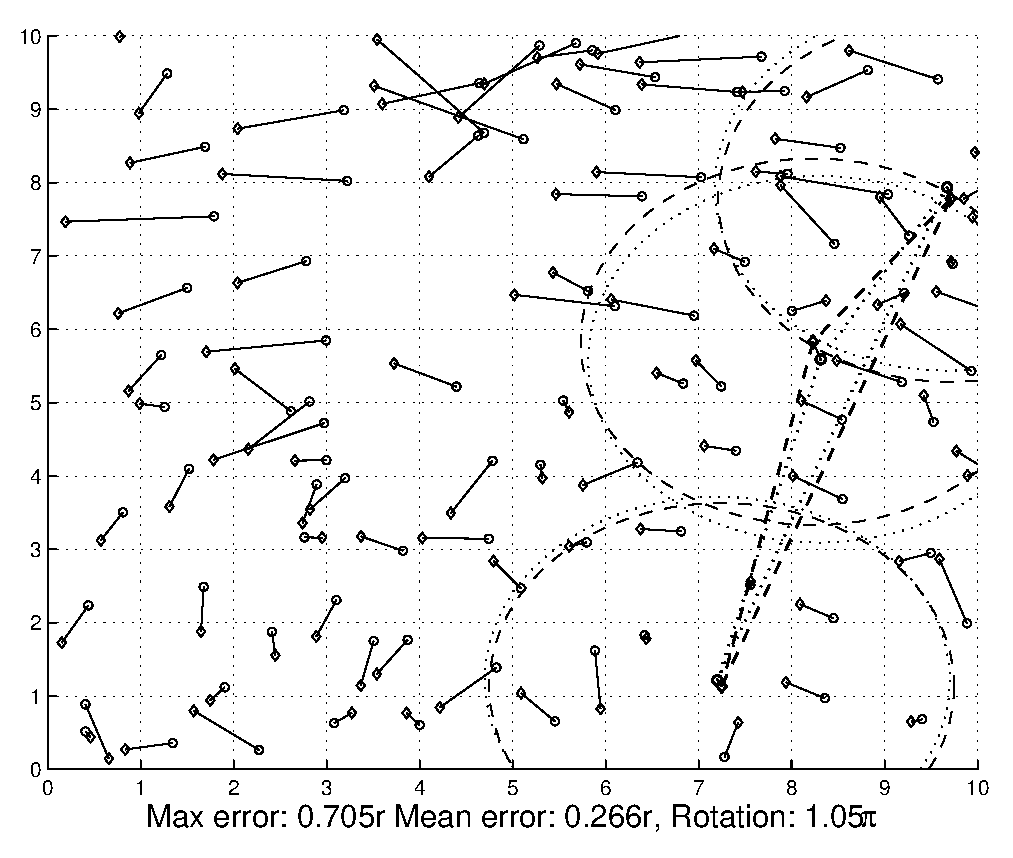
\includegraphics[width=\figurewidth\textwidth]{outliers/AS6/AS6NetworkDiff7}}
	\\
	\subfloat[Network B]{\label{fig:AS6NetworkDiff10}
		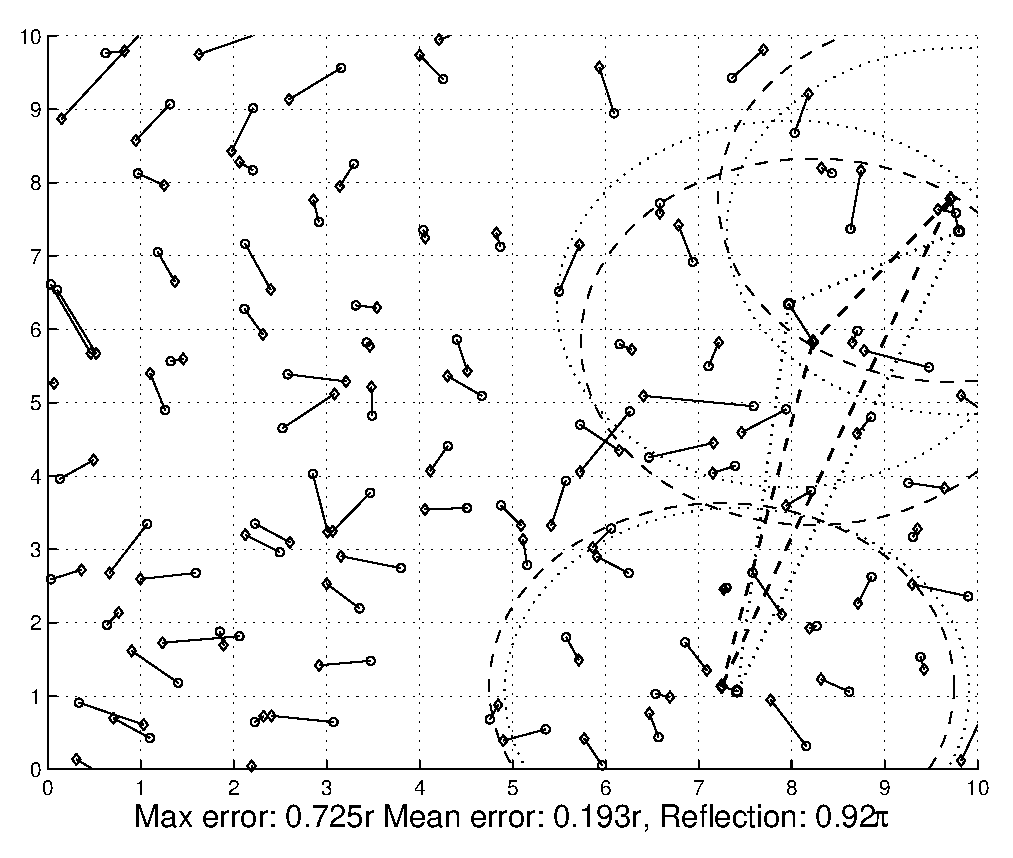
\includegraphics[width=\figurewidth\textwidth]{outliers/AS6/AS6NetworkDiff10}}
	\caption{Good localization performance with same anchor set in two different networks}
	\label{fig:AS6good}
\end{figure}

Further, Figures~\ref{fig:AS6bad1} and \ref{fig:AS6bad2} show two more random networks, using the same anchor set as above.  As seen in Chapter~\ref{chap:outliers}, some short anchor node triangles can cause extremely poor localization.  In this case, we see that even the same anchor set does not necessarily mean that the resulting localization results will be so poor.  

\begin{figure}
  \centering
	\subfloat[Network C]{\label{fig:AS6NetworkDiff9}
		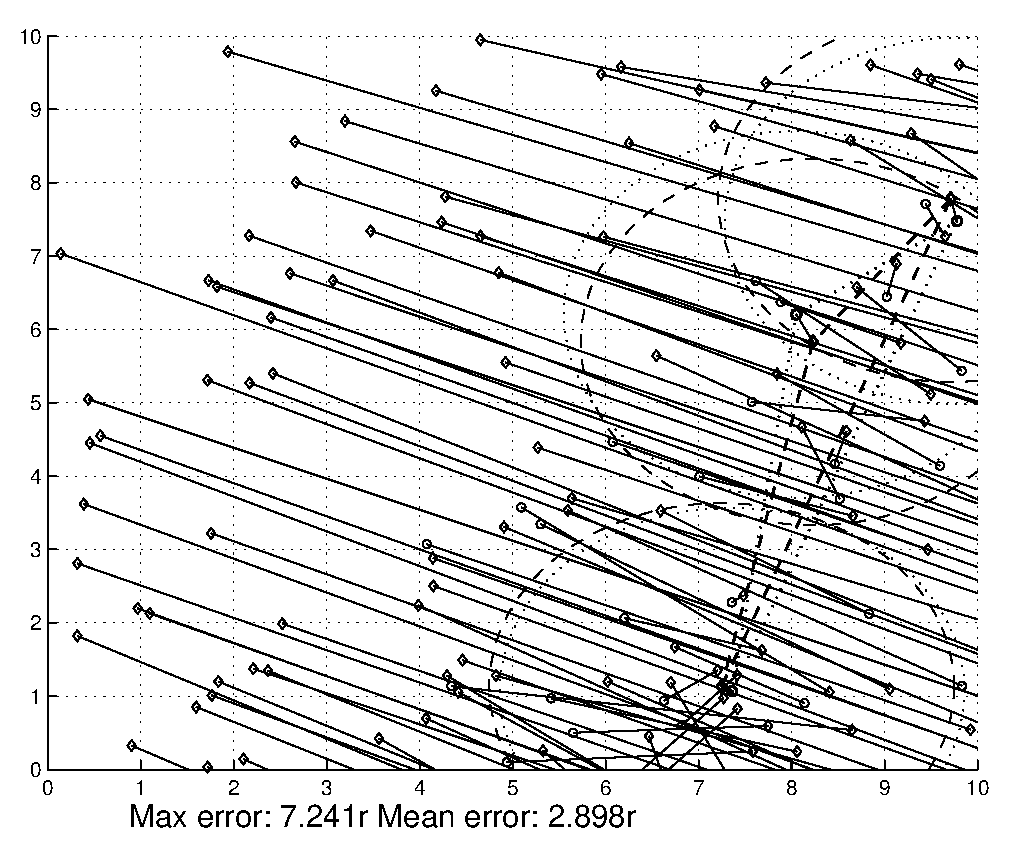
\includegraphics[width=\figurewidth\textwidth]{outliers/AS6/AS6NetworkDiff9}}
\\
	\subfloat[Network D]{\label{fig:AS6NetworkDiff8}
		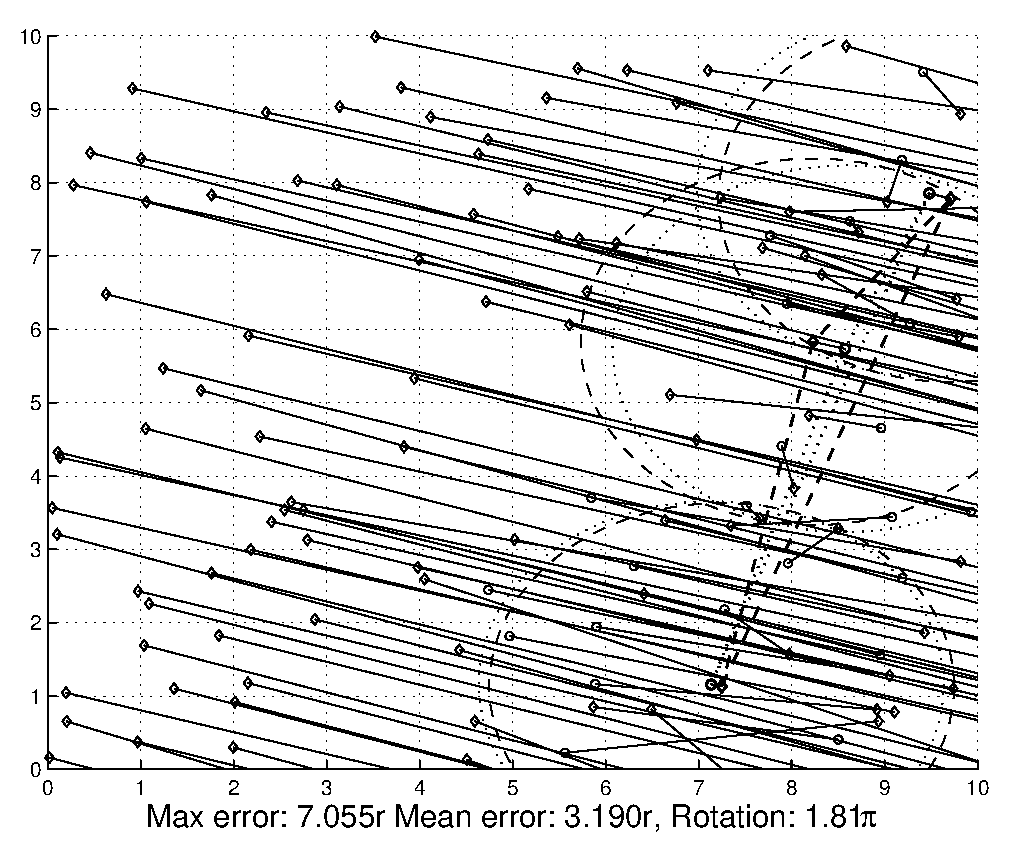
\includegraphics[width=\figurewidth\textwidth]{outliers/AS6/AS6NetworkDiff8}}	
    \caption{Poor localization performance with same anchor set in two different networks}
	\label{fig:AS6bad}
\end{figure}

\section{Node Distance from the Anchors}

Of great assistance to network designers would be to know where in the network nodes are expected to have poor localization performance.  With this information, and if the anchor placement is somewhat constrained, they could either avoid placing nodes in the expected poor area, or take into account the higher expected localization errors in the analysis of the data.

Figure~\ref{fig:AS6goodcontour} shows the same network and anchor sets as in Figure~\ref{fig:AS6good}, but instead of showing a line representing the localization errors, the error at each point is taken and a grid of location errors is then interpolated throughout the area of the network.  A contour plot based on that interpolated grid is then shown in the figure.  The goal in viewing this network map is to attempt to discover a pattern in terms of the relationship of a an area of the network to the location of the anchor nodes themselves.  Unfortunately, no geographic correlation can be ascertained.

\begin{figure}
  \centering
	\subfloat[Network A]{
		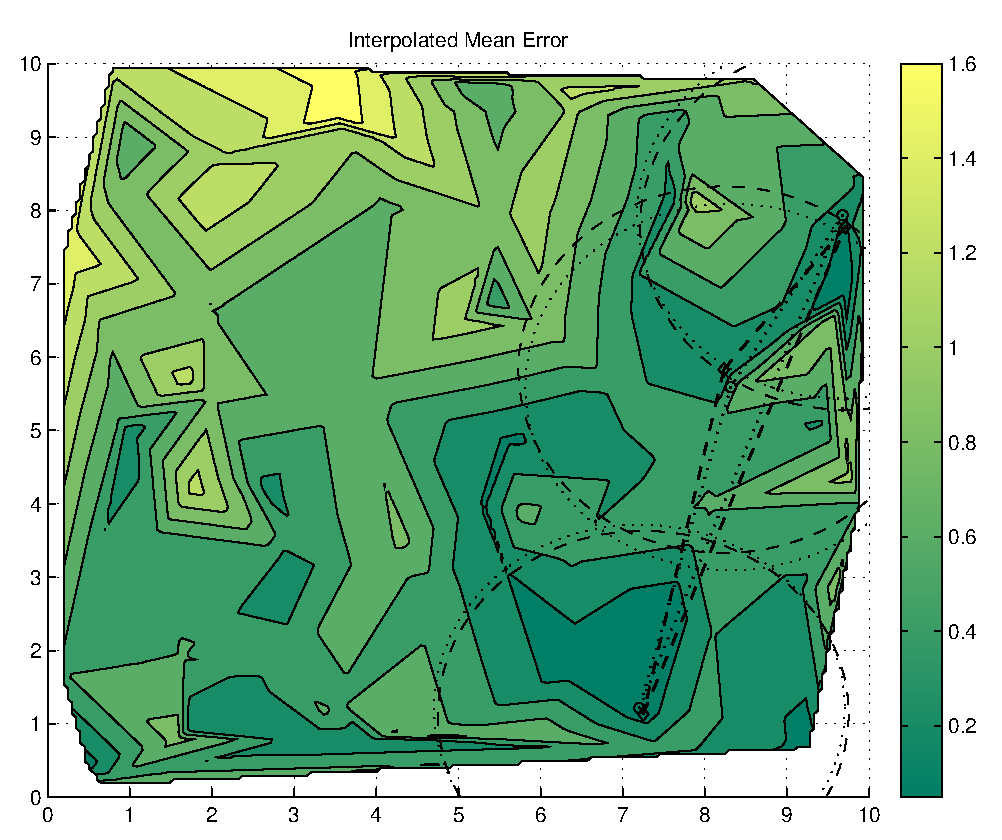
\includegraphics[width=\figurewidth\textwidth]{outliers/AS6/AS6NetworkContour7}}
	\\
	\subfloat[Network B]{
		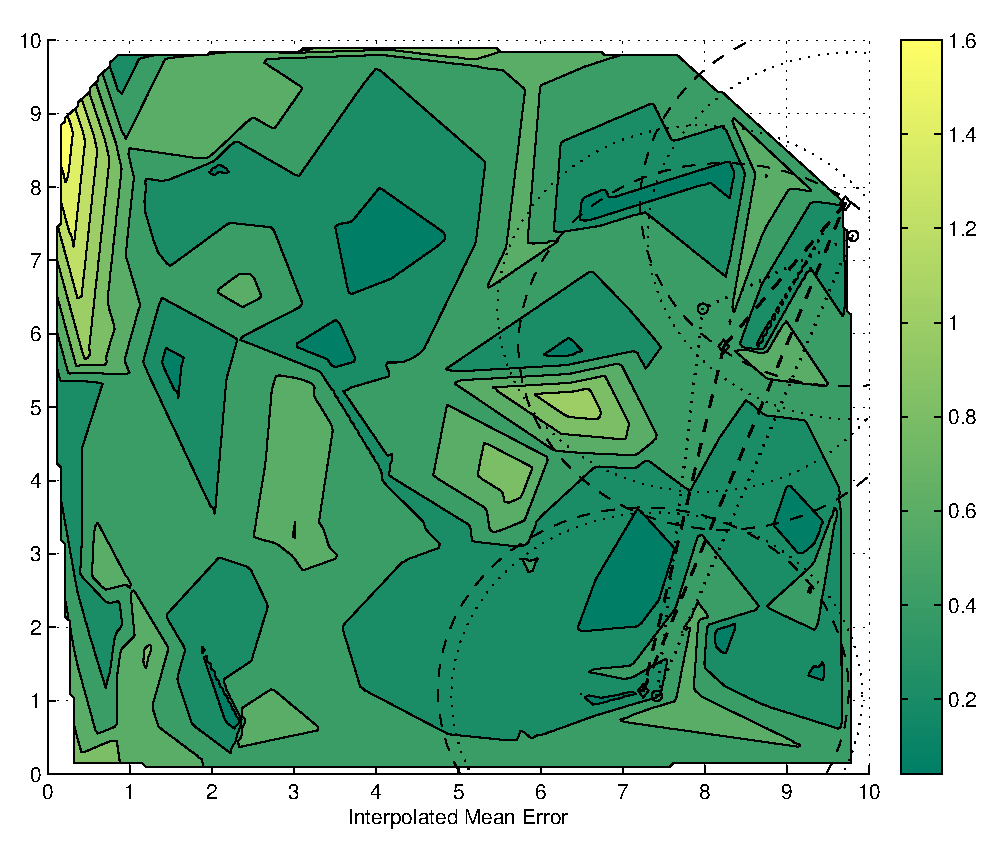
\includegraphics[width=\figurewidth\textwidth]{outliers/AS6/AS6NetworkContour10}}
	\caption{Localization error as a contour plot}
	\label{fig:AS6goodcontour}
\end{figure}


\section{Applicability to Varying Network Topology}
